\subsection{Background Scene Visualization}
In this section, 185 pictures of garden(picking $\frac{1}{4}$ of the original resolution for efficiency) are trained. It takes about \textbf{1:12:42hour} to extract pose with COLMAP and \textbf{19:30min}(20000 epochs) to train.

One of the original pictures and the rendering results are as follow:
\begin{figure}[H]
	\centering
	

	\begin{subfigure}{0.25\textwidth}
		\centering
		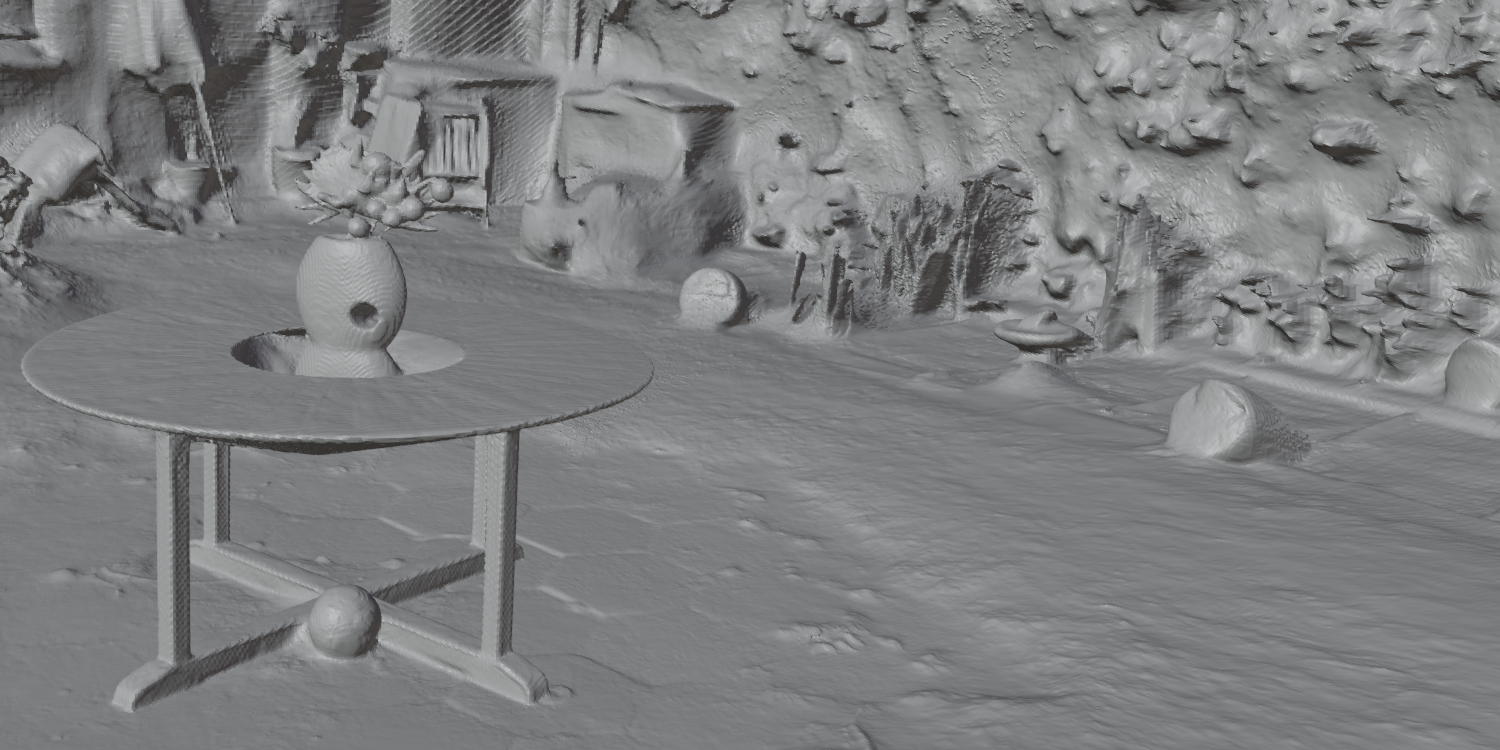
\includegraphics[width=\linewidth]{figures/task1/background/garden_mesh.png}
		\caption{Garden Mesh}
	\end{subfigure}
	\hfill
	\begin{subfigure}{0.25\textwidth}
		\centering
		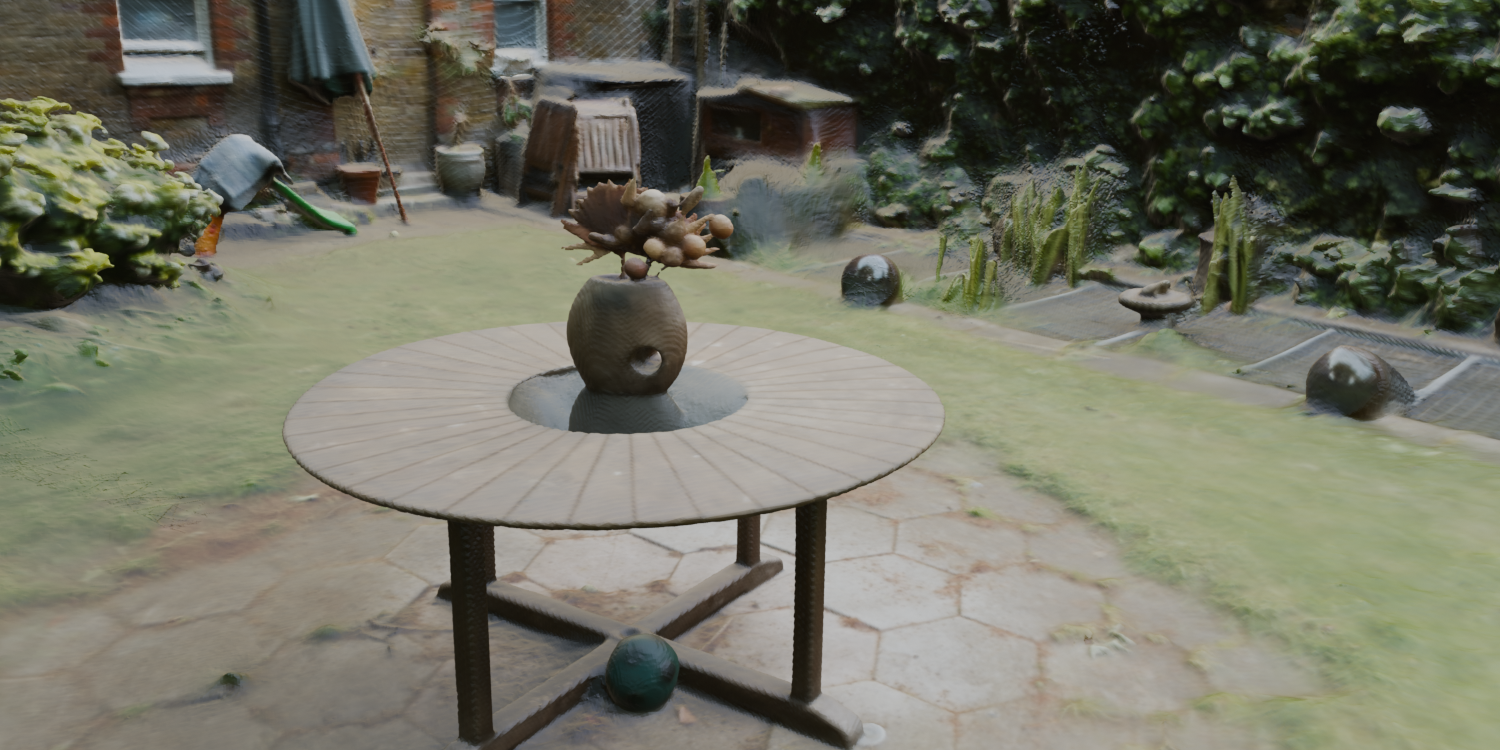
\includegraphics[width=\linewidth]{figures/task1/background/garden_color.png}
		\caption{Garden Color}
	\end{subfigure}
	\hfill
	\begin{subfigure}{0.25\textwidth}
		\centering
		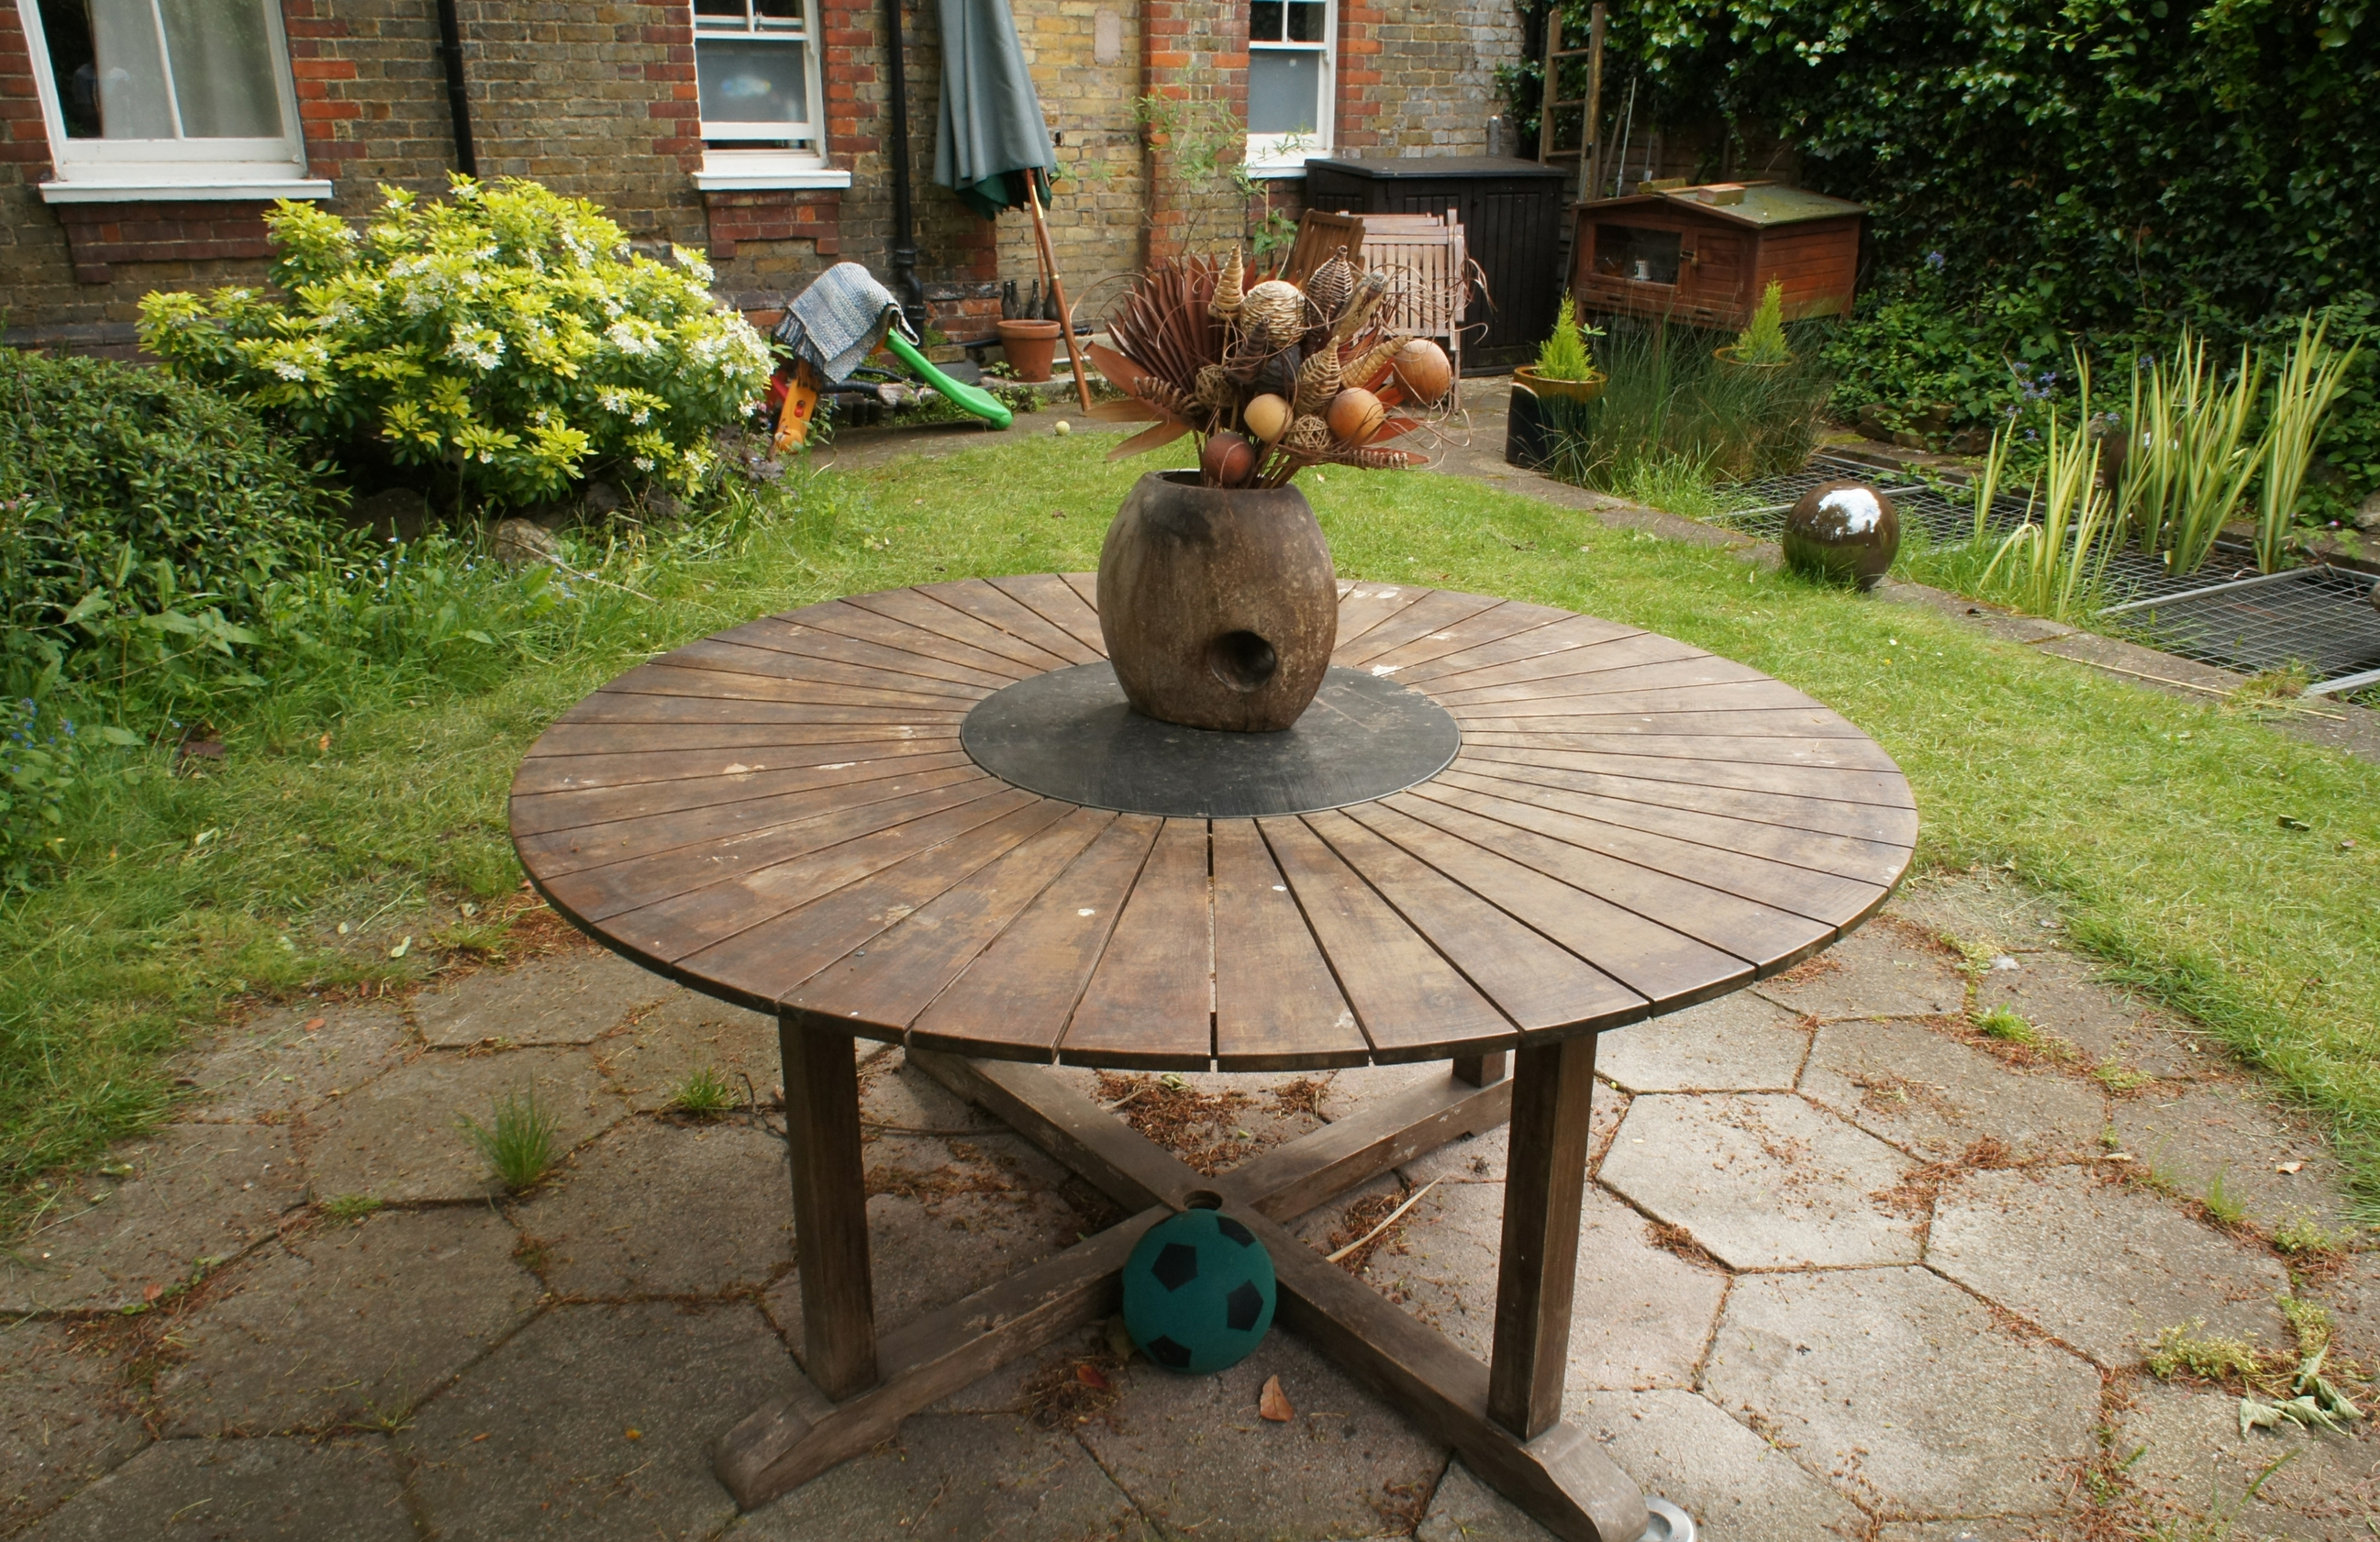
\includegraphics[width=\linewidth]{figures/task1/background/garden.jpg}
		\caption{Original Garden}
	\end{subfigure}
	
	\vspace{0.6cm}
	
	
\end{figure}
In this part, 2 meshes are exported(bounded and unbounded), where the unbounded mesh is in a form of a whole box. The box has an irregular outer shell and sky because these parts are not included in the images, while the rest of the model looks very good.


The detailed quality analysis will be shown later.



The training dynamics are as follow:

\begin{figure}[H]
	\centering
	
	% 第一行
	\begin{subfigure}{0.4\textwidth}
		\centering
		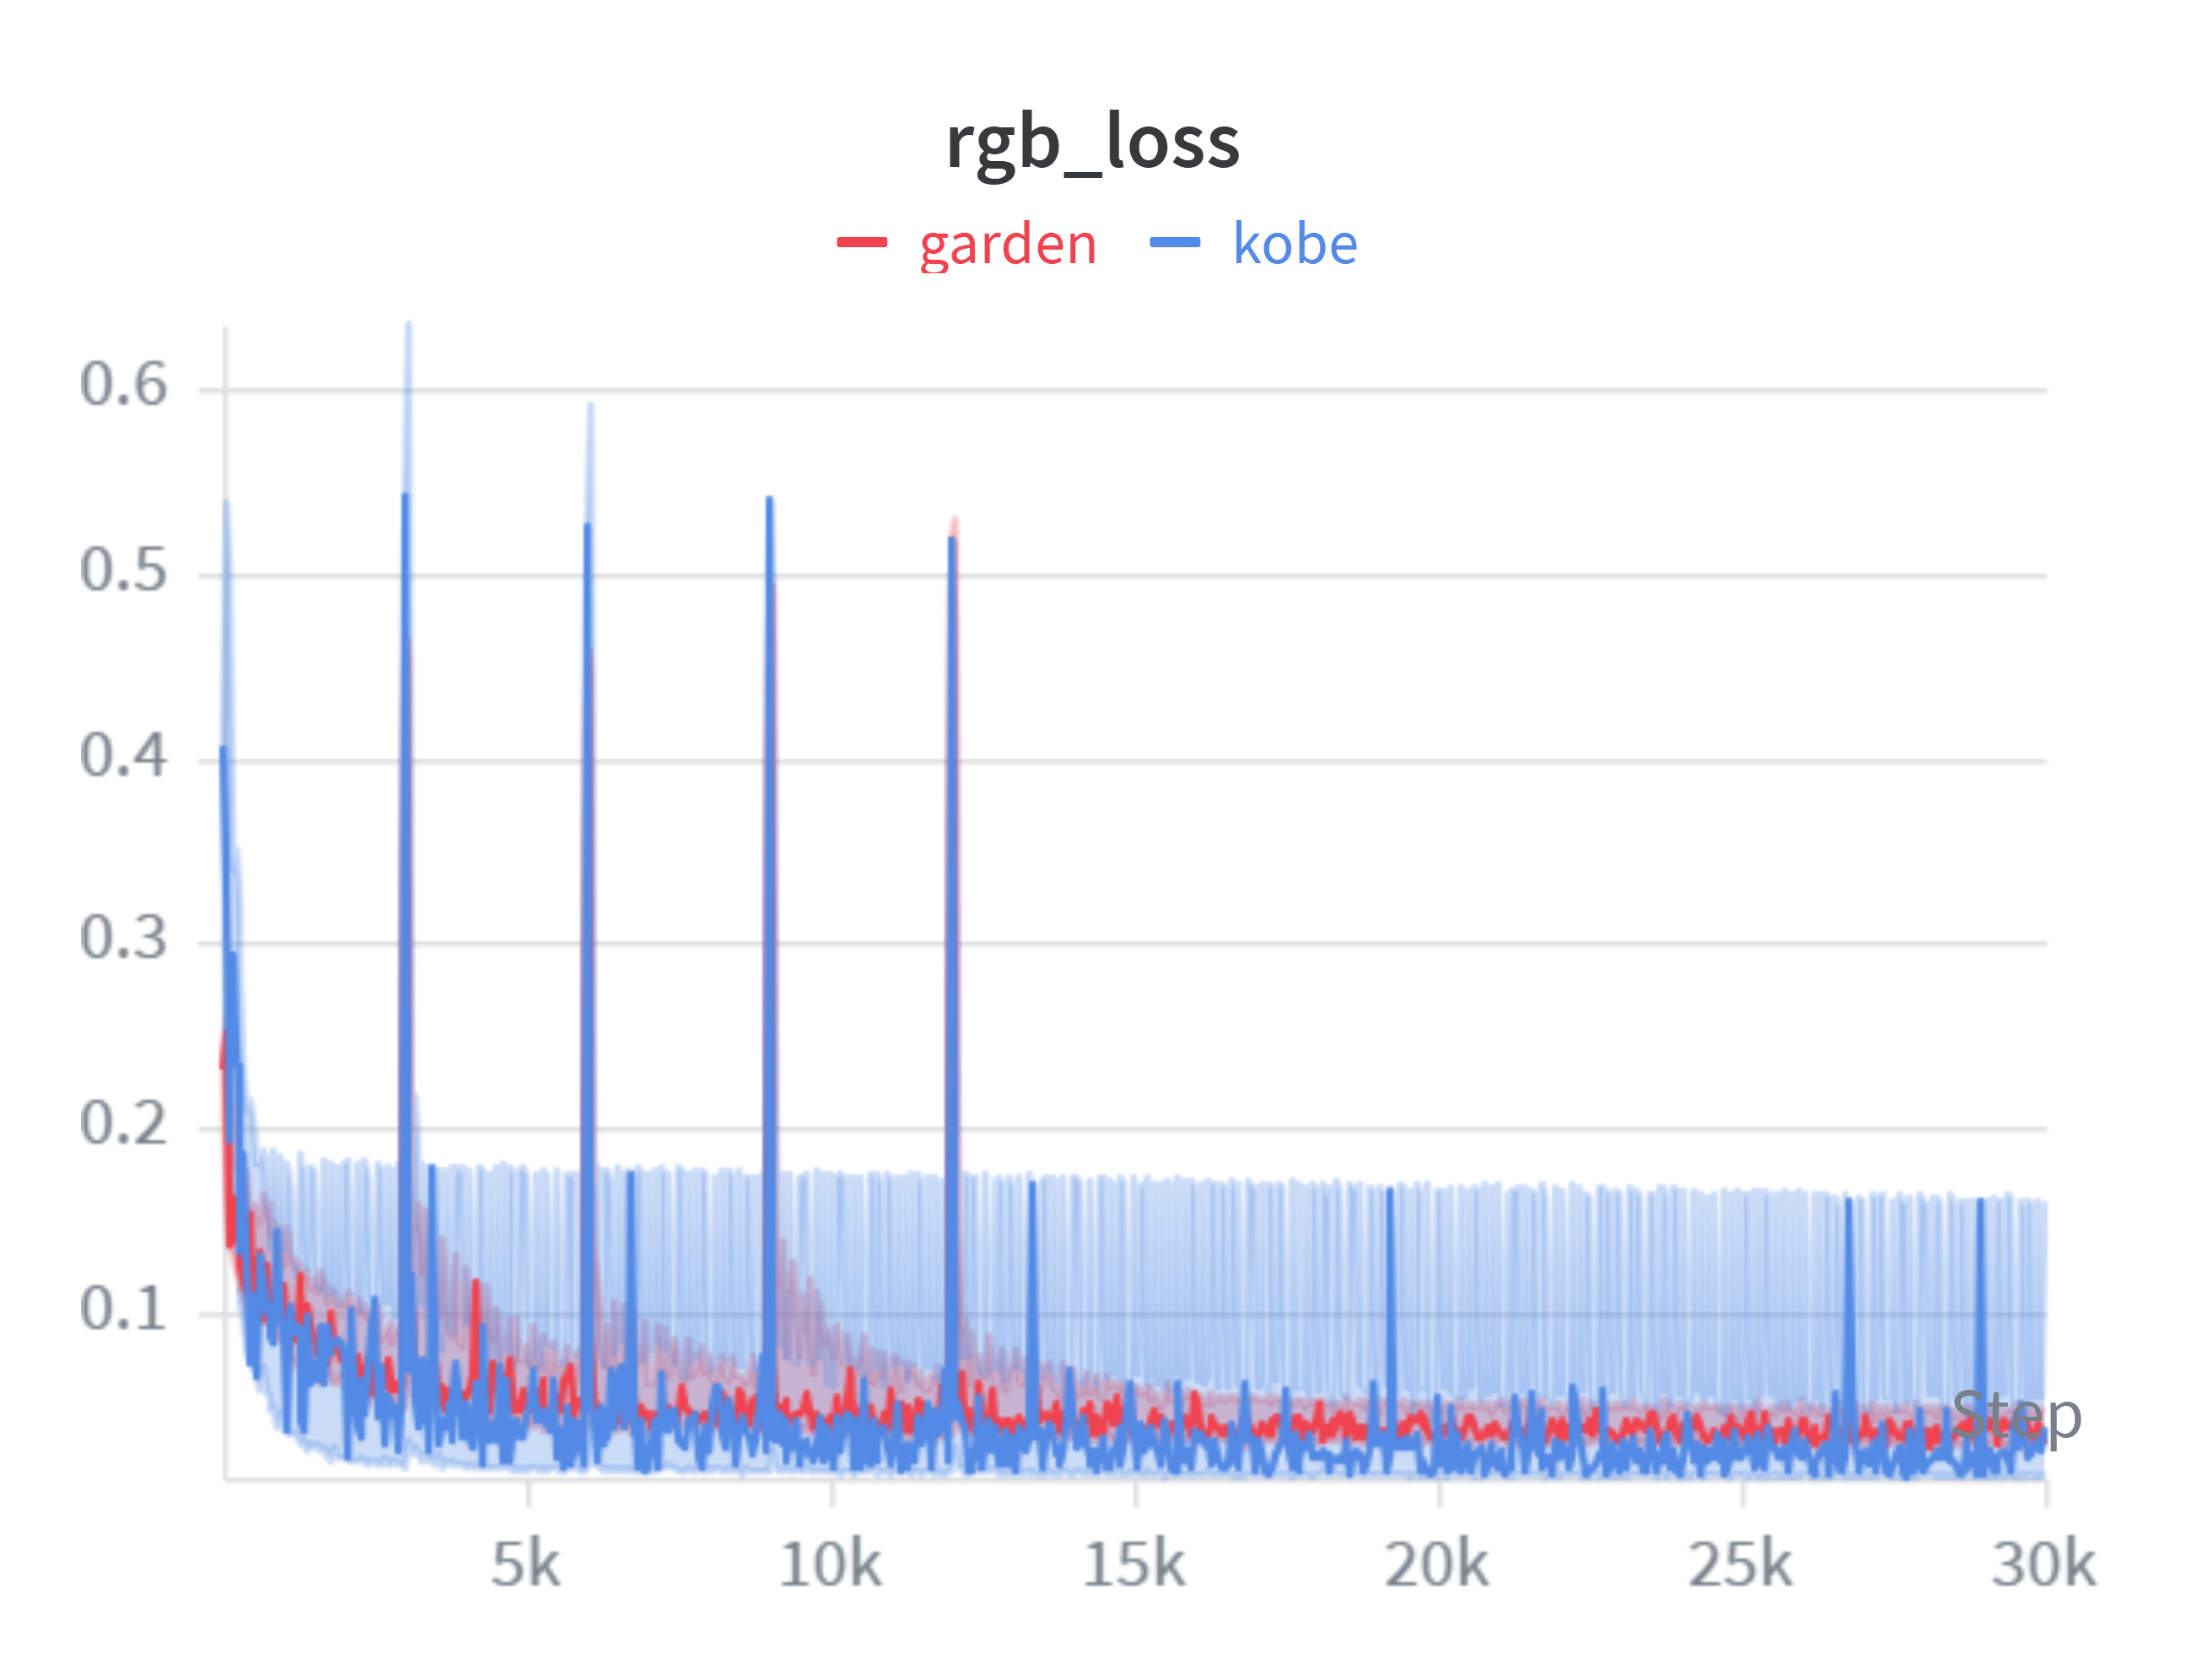
\includegraphics[width=\linewidth]{figures/task1/background/rgb_loss.png}
		\caption{RGB Loss}
	\end{subfigure}
	\hfill
	\begin{subfigure}{0.4\textwidth}
		\centering
		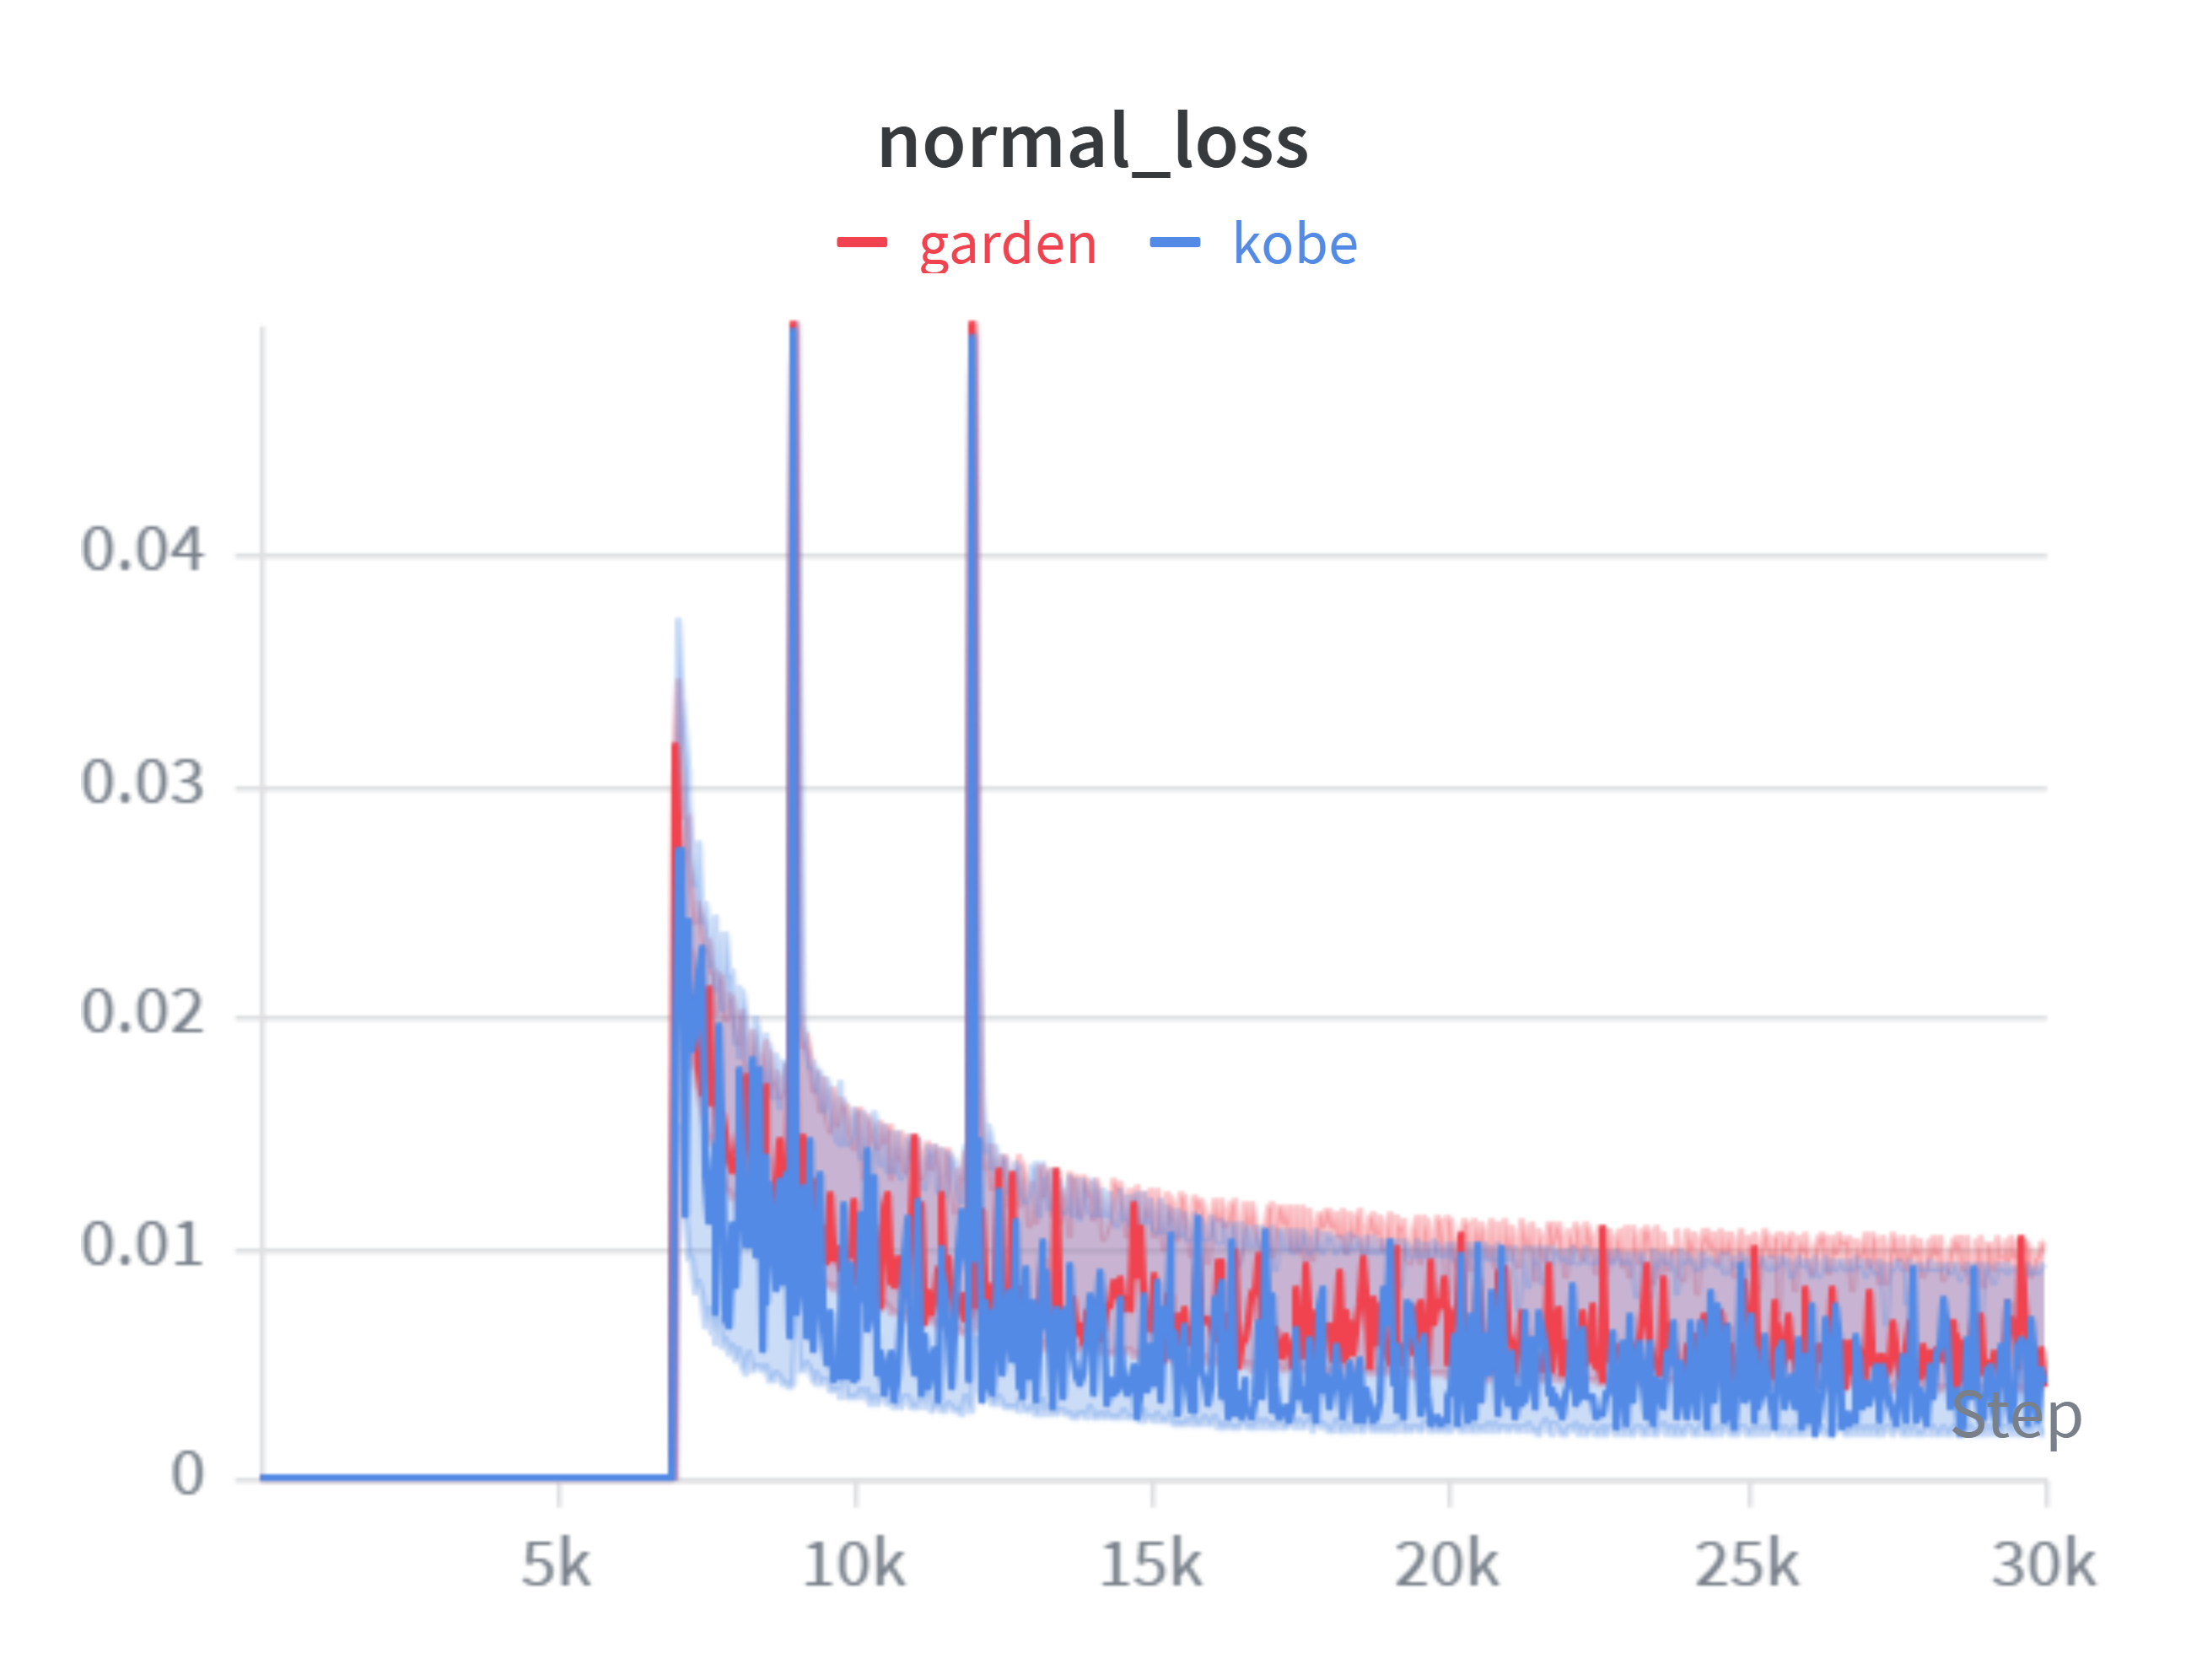
\includegraphics[width=\linewidth]{figures/task1/background/normal_loss.png}
		\caption{Normal Loss}
	\end{subfigure}

	
	\caption{Training Dynamics}
	\label{fig:2DGS Dynamics}

\end{figure}

Both loss curves generally show a downward trend, and the red curve (Garden) is more stable and has fewer peaks than the blue curve (Kobe). This is likely because the Garden has 185 images, twice the dataset of Kobe, thus capturing color and normal information more accurately. Also, Garden captures way more feature points after COLMAP as is shown in Figure~\ref{figure:Feature Points}




